% VUT FIT MITAI
% MSZ 2021/2022
% Author: Vladimir Dusek
% Login: xdusek27

%%%%%%%%%%%%%%%%%%%%%%%%%%%%%%%%%%%%%%%%%%%%%%%%%%%%%%%%%%%%%%%%%%%%%%%%%%%%%%%%

% Path to figures
\graphicspath{{pdi/konzistentni_globalni_stav/figures}}

%%%%%%%%%%%%%%%%%%%%%%%%%%%%%%%%%%%%%%%%%%%%%%%%%%%%%%%%%%%%%%%%%%%%%%%%%%%%%%%%

\chapter{PDI -- Podmínky konsistentního globálního stavu distribuovaného systému.}

% Todo:
% - Chtelo by to pravdepodobne doplnit i algoritmy pro dosazeni konzistentniho stavu.

%%%%%%%%%%%%%%%%%%%%%%%%%%%%%%%%%%%%%%%%%%%%%%%%%%%%%%%%%%%%%%%%%%%%%%%%%%%%%%%%

\subsection{Metadata}

\begin{compactitem}
    \item Předmět: Prostředí distribuovaných aplikací (PDI)
    \item Přednáška:
    \begin{compactitem}
        \item 4) Globální stav a snapshots
    \end{compactitem}
    \item Záznam:
    \begin{compactitem}
        \item 2020-10-12
    \end{compactitem}
\end{compactitem}

%%%%%%%%%%%%%%%%%%%%%%%%%%%%%%%%%%%%%%%%%%%%%%%%%%%%%%%%%%%%%%%%%%%%%%%%%%%%%%%%

\section{Úvod a kontext}

\paragraph*{Distribuovaný systém} Distribovaný systém je množina procesů $p_1, p_2, \dots, p_n$, které jsou propojeny komunikačními kanály. V~systému neexistuje žádná globální paměť ani globální hodiny. Procesy spolu komunikují pouze zasíláním zpráv skrze komunikačními kanály.

\paragraph*{Komunikační kanál} Komunikační kanál mezi procesy $p_i$ a $p_j$ značíme $C_{ij}$.

\paragraph*{Událost} Rozlišujeme tři typy událostí: interní událost procesu, zaslání zprávy a přijetí zprávy.

\paragraph*{Zpráva} Zpráva $m_{ij}$ značí zprávu zaslanou procesem $p_i$ procesu $p_j$. $send(m_{ij})$ značí odeslání zprávy a $recv(m_{ij})$ přijetí.

\paragraph*{Stav procesu} Lokální stav procesu $p_i$ značíme $LS_i$. Lokální stav je definován jako sekvence všech událostí, o~kterých proces $p_i$ ví. Nechť $e$ je libovolná událost, $e \in LS_i$ značí, že událost $e$ patří do lokálního stavu procesu $p_i$, $e \not\in LS_i$ značí, že událost $e$ nepatří do lokálního stavu procesu $p_i$.

\paragraph*{Stav komunikačního kanálu} Stav komunikačního kanálu $C_{ij}$ značíme $SC_{ij}$ a je definován množinou zpráv, které obsahuje. Pro kanál $C_{ij}$ můžeme definovat jeho stav na základě lokálních stavů procesů $LS_i$ a $LS_j$: $$
transit(LS_i, LS_j) = \{ m_{ij} \,|\, send(m_{ij}) \in LS_i \land rec(m_{ij}) \not\in LS_j \}
$$.

\section{Model komunikace}

\begin{compactitem}
    \item FIFO -- Komukační kanál funguje jako fronta zpráv \textit{first in}, \textit{first out}. Kanál tedy zachovává pořadí zpráv sám o~sobě.

    \item non-FIFO -- Komunikační kanál se chová jako datová struktura množina, do které odesílatel vkládá zprávy a příjemce je odebírá v~náhodném pořadí.

    \item Causal ordering (kauzální uspořádání) -- Systém, který podporuje kauzální doručení zpráv splňuje následující vlastnost. Pro jakékoliv dvě zprávy $m_{ij}$ a $m_{kj}$ platí, pokud $send(m_{ij}) \rightarrow send(m_{kj})$, pak i $recv(m_{ij}) \rightarrow recv(m_{kj})$.
\end{compactitem}

\section{Konzistentní globální stav}

\paragraph*{Globální stav} Globální stav distribuovaného systému je kolekce lokálních stavů procesů a komunikačních kanálů. $$
GS = \Big\{ \bigcup_{i} LS_i \,,\, \bigcup_{i, j} SC_{ij} \Big\}
$$.

\paragraph*{Časoprostorový diagram} Diagram pro vizualizaci komunikace procesů v~distribuovaném systému. Viz obrázek~\ref{48_example_cut} a~\ref{48_example_consistent_state}.

\paragraph*{Konzistentní globální stav} Konzistentní globální stav (\textit{snapshot}) je stav systému v~určitém časovém okamžiku. Lze si jej představit jako řez v~časoprostorovém diagramu, který rozděluje diagram na dvě části: minulost a budoucnost. Aby byl řez (globální stav) konzistentní, tak pokud je doručení nějaké zprávy v~minulosti, musí být v~minulosti i její odeslání. Formálně jde o~globální stav, který splňuje nálsedující podmínky:

$$
send(m_{ij}) \in LS_i \Rightarrow m_{ij} \in SC_{ij} \oplus recv(m_{ij}) \in LS_j
$$,

$$
send(m_{ij}) \not\in LS_i \Rightarrow m_{ij} \not\in SC_{ij} \land recv(m_{ij}) \not\in LS_j
$$.

\paragraph*{K čemu je \textit{snapshot}} \textit{Snapshot} lze využít např. pro tvorbu záloh systému nebo při zotavování systému po chybách.

\paragraph*{Jak lze \textit{snapshot} vytvořit} Absence globální sdílené paměti, globálních hodin a nepředvídatelná délka zpoždění v~odesílání zpráv v~distribuovaném systému činí problém vytváření snapshotů netriviálním. Způsob vytváření lze rozdělit do dvou kategorií: na základě algoritmů a na základě checkpointů.

\paragraph*{Problémy při zaznamenávání snapshotu} Jak rozlišit mezi zprávami, které mají být součástí snapshotu a které nikoliv?
\begin{compactitem}
    \item Zprávy, které jsou odeslány procesem před zaznamenáním svého  snapshotu, jsou zaznamenány do stavu.
    \item Zprávy, které jsouodeslány procesem po zaznamenání svého  snapshotu, nejsou zaznamenány do stavu.
\end{compactitem}

\noindent Jak rozpoznat okamžik, ve kterém má proces zaznamenat snapshot?
\begin{compactitem}
    \item Proces $p_j$ musí zaznamenat svůj snapshot před zpracováním zprávy $m_{ij}$, která byla poslána procesem $p_i$ po zaznamenání jeho snapshotu.
\end{compactitem}

\begin{figure}[H]
    \centering
    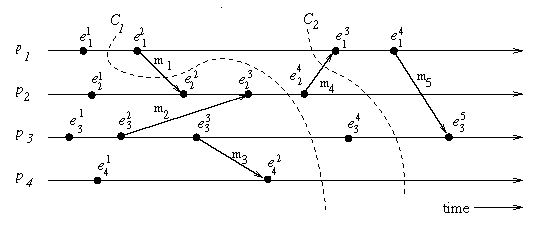
\includegraphics[width=1\linewidth]{example_cut.pdf}
    \caption{Příklad řezu v~časoprostorovém diagramu. Řez $C_1$ je nekonzistentní, kvůli zprávě $m_1$. Řez $C_2$ je konzistentní a zpráva $m_4$ je zachycena ve stavu kanálu $Ch_{21}$.}
    \label{48_example_cut}
\end{figure}


\begin{figure}[H]
    \centering
    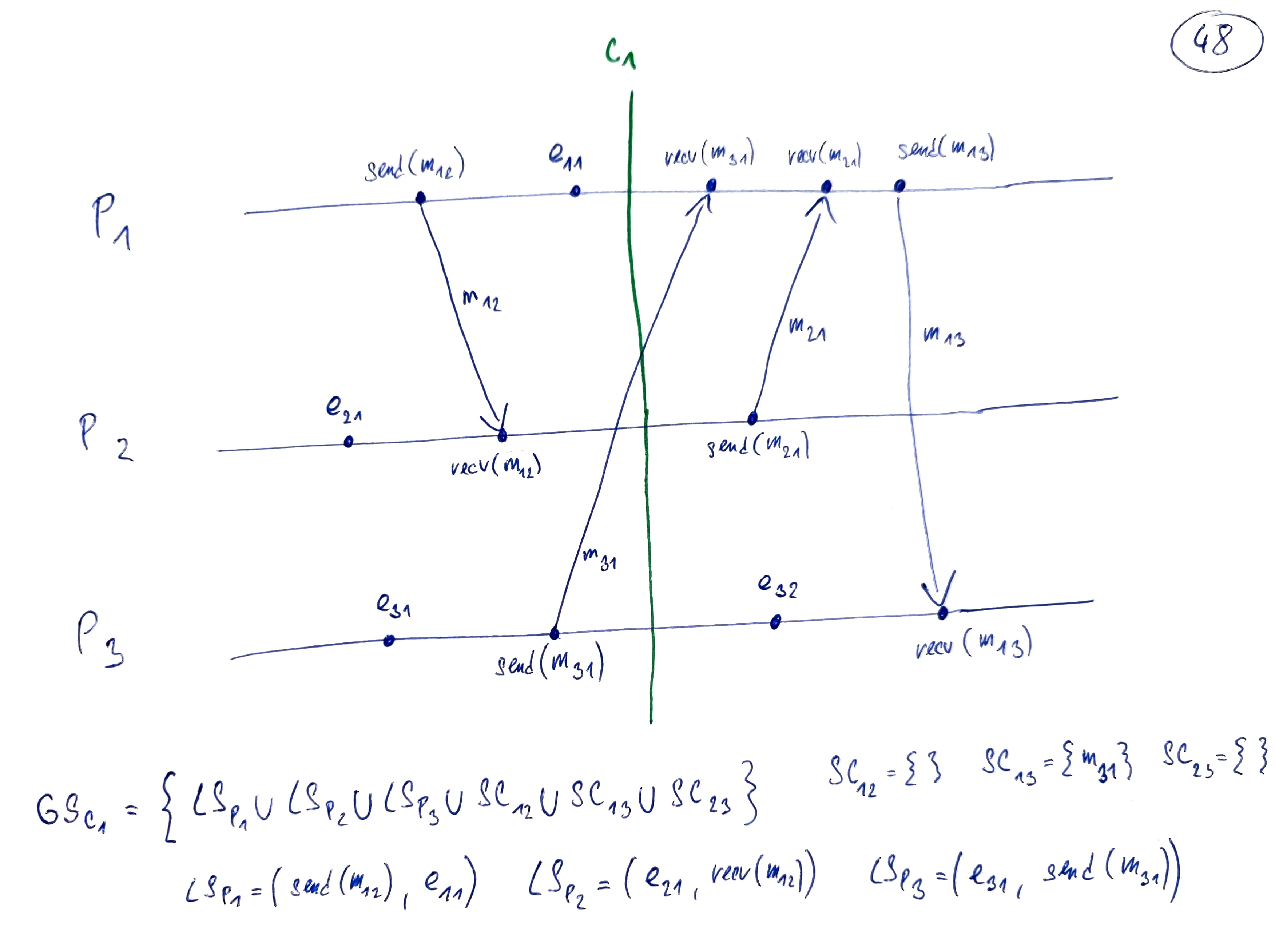
\includegraphics[width=1\linewidth]{example_consistent_state.pdf}
    \caption{Příklad konzistentního globální stavu formálně.}
    \label{48_example_consistent_state}
\end{figure}
